% [max 300 words]
% how is the tool used, elaborate on a use case what can be achieved with the tool (mainly use screenshots?)
The easy-to-use nature of the application originates from its linear flow of instructions and capabilities. The user can, for example, not start to try to sniff packets or inject something in an \texttt{img}-tag when the ARP-cache poisoning thread has not been configured and started yet (i.e. no man-in-the-middle position). In particular, the user is lead through the following chain of exploitations, configurations and (possible) attacks: Local Network Scan $\,\to\,$ ARP Cache Poisoning $\,\to\,$ Injections and Extractions.

\begin{figure}[h!]
	\centering
	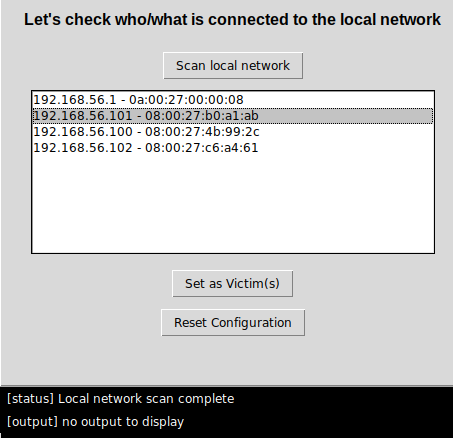
\includegraphics[width=0.5\textwidth]{img/network_scan.png}
	\caption{
		The network scan as is facilitated to the end-user}
	\label{fig:gui_network_scan}
\end{figure}

A user can perform the ARP Cache Poisoning without a local network scan (i.e. specifying the target/victim IP's himself), but execution of ARP Cache poisoning and a Local Network Scan are  preconditions for the injections and extractions. The first condition is rather trivial (mitm). The latter condition is needed to have a full map of all the IP-addresses to their respective MAC-addresses. The ARP Cache poisoning is possible on its own since it only requires the user's own mac-address (automatically retrieved in the application) and the target and victim IP'. We need to know the real mac-addresses of our victims for the injections and extractions (e.g. for packet sniffing, modification and -forwarding).\\ 

\begin{figure}[t!]
	\centering
	\begin{subfigure}{0.51\textwidth}
	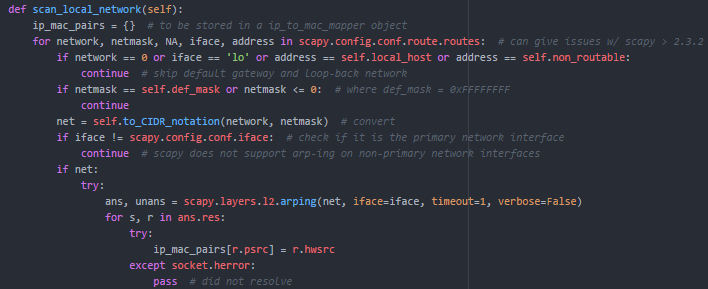
\includegraphics[width=\textwidth]{img/network_discoverer.png}
		\caption{A snippet from the source-code of the network discoverer}
	\end{subfigure}

	\begin{subfigure}{0.51\textwidth}
		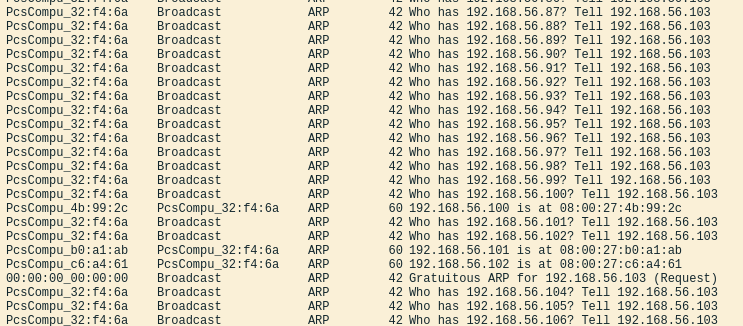
\includegraphics[width=\textwidth]{img/wireshark_network_scan}
		\caption{The ARP requests from our local network scanner in Wireshark}
	\end{subfigure}
\caption{
	Network scan in the GUI and Wireshark}
	\label{fig:network_scan}
\end{figure}

A snippet of the source code (see comments in the source code) of one of the core functionalities of our network discoverer is depicted in \autoref{fig:network_scan}. The code is rather self-explanatory. The ARP-requests can also be observed in Wireshark. This should gives you an easy to digest visualization of what is being done in the iterations of the source code (see incremental IP-addresses). The next step is the actual spoofing. If the user has selected the target and victim(s) in the list, they will be automatically loaded in the next tab \autoref{fig:arp_spoof}. ARP spoofing is done on a separate thread which keeps poisoning (10 second interval) as long the thread is alive as can be seen in the source code.\\

\begin{figure}[t!]
	\centering
	\begin{subfigure}{0.51\textwidth}
	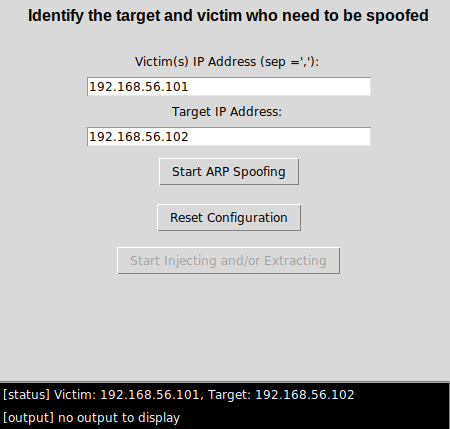
\includegraphics[width=\textwidth]{img/arp_spoofing.png}
		\caption{The ARP spoofing tab in the GUI}
	\end{subfigure}

	\begin{subfigure}{0.51\textwidth}
		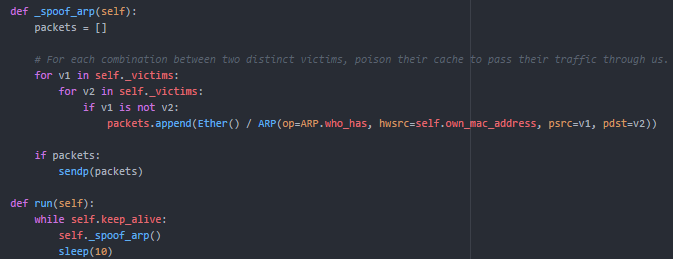
\includegraphics[width=\textwidth]{img/arp_spoof_code}
		\caption{The core functionality of the ARP-spoofing class (inherits threading.Thread)}
	\end{subfigure}
\caption{
	ARP spoofing in the GUI and source code}
	\label{fig:arp_spoof}
\end{figure}


\newpage 
Note that in the previous step the button that leads to the injection and extraction tab is still disabled. Once the `Start ARP spoofing' button is clicked one is redirected to the most fun and resourceful tab. We can see this tab in \autoref{fig:injection_filtering} where the cookie-filter has been turned on and a dummy attack has been displayed. For some extractors/filters and injectors, like the TCP regular-expression filter and \texttt{img}-tag injector, user input is needed which the user can specify in the input box that pops-up in the GUI.\\

\begin{figure}[t!]
	\centering
	\begin{subfigure}{0.45\textwidth}
	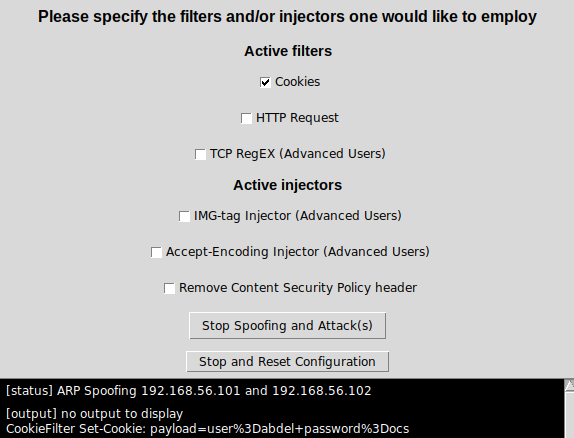
\includegraphics[width=\textwidth]{img/injection_filtering.png}
		\caption{The tab where all the injectors and filters are facilitated. Note that this is just a snippet. The output and status frame are significantly larger in the application. In addition, one can go to a previous step in the tab-navigation based GUI}
	\end{subfigure}

	\begin{subfigure}{0.45\textwidth}
		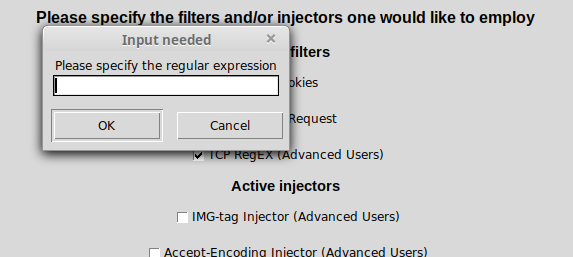
\includegraphics[width=\textwidth]{img/tcp_reg_ex.png}
		\caption{User input has to be given for some functionalities}
	\end{subfigure}
\caption{
	Extractors and Injectors}
	\label{fig:injection_filtering}
\end{figure}

The code for filters/extractors and injectors can be found in our repository (\href{https://github.com/akbokha/fhttp}{\texttt{fHTTP}'s GitHub page}). A lot emphasis and effort is put on modularity, abstraction, adhering to overall design principles and minimization of dependencies and various other (core) software engineering principles. Introducing new filters/extractors, by other contributors since it is an open-source project, is for example made easy by the facilitation of abstract classes.